\documentclass{article}
\usepackage[letterpaper,portrait,margin=1in]{geometry}
\usepackage{amsfonts}
\usepackage{amsmath}
\usepackage{array}
\usepackage{hhline}
\usepackage{tikz}
\usepackage{hyperref}
\setlength\parindent{0pt}

\begin{document}
	
\title{Supplement}
\date{\vspace{-5ex}}
\maketitle

\tableofcontents

\section{Results}

We developed a C++ code base for cell-based modelling as described in the methods section. This model simulates cell growth among multiple cell types. The cellular mechanics are adapted from Drasdo-Hohme ... [citation]. Building from their paper, our model has the following critical parameters related to cell growth...

To determine which of these parameters impact phenotype, we peformed the following senstivity analysis.

\section{Methods}

\subsection{Model Description}

The model used in this paper was implemented with an R package, \textit{CancerInSilico}. It is a cell-based, off-lattice model based on the work of ... [citation]. While the underlying model does not contain any novel mechanisms, using it as a basis for simulating gene expression data is a new approach.

\subsubsection{Cell Mechanics}

There are two primary components of a cell-based model that determine cell mechanics: the geometrical structure of the cells and the process by which cells move and grow [citation]. In an off-lattice model, cells are typically represented by their coordinates and volume. Our implementation assumes that cells are spherical - in two dimensions this equates to a point mass with some radius. Having a fixed volume is not always neccesary in an off-lattice model (see spring model [citation]), but we find it to be a convenient attribute. The radius of a cell allows for strict adherence to the 'excluded volume effect' and allows for an easily interpretable notion of cell size [citation]. The mechanics of a cell during division differ slightly from those of a normal cell. At the time of division cells deform into a 'dumbell' shape, eventually separating into a daughter and parent cell (see Supp) [citation]. While the cell is in this shape, excluded volume interactions still occur, but now there are two centers of the cell to account for (see Supp).\\
\\
The geometry of cells in an off-lattice model provide the core structure, but the updating procedure is responsible for actually enforcing the desired cell mechanics. In our implemention we use a  monte-carlo approach to update the cells [citation]. At each monte carlo step, a cell is chosen randomly and a change is proposed. For cells in division the possible changes are rotate, move, and deform. For cells not in division the possible changes are either grow or move. Each state change is proposed with some probability and accepted with some probability. The proposal probabilities are input parameters to the model and the acceptance probabilities are determined by attempting to minimize some "total energy" function. In this way the model is similiar to some models in physics (see Ising model). The total energy function allows for a high level summary of what general cell-cell interactions should look like. In our implementation we use the following [citation]\\
\\
$V^{tot} = \sum_{i<j} V_{ij}$\\
\\
$V_{ij} =
\left\{
\begin{array}{ll}
      \Bigr(\dfrac{2d_{ij}}{\delta} - 1\Bigr)^2 - 1 & 0 \leq d_{ij} \leq \delta \\
      \infty & otherwise \\
\end{array} 
\right. $\\
\\
$d_{ij} = $ distance between cells $i$ and $j$.\\
\\
\\
\\
Changes are accepted with probability:\\
\\
$P_{accept} = 
\left\{
\begin{array}{ll}
    e^{-\epsilon\Delta V^{tot}} & \Delta V^{tot} \geq 0 \\
    1 & \Delta V^{tot} < 0 \\
\end{array} 
\right. $\\
\\
This simple energy function enforces cell-cell adhesion and provides the cells enough room to grow. Cells are in the ideal configuration when $d_{ij} = \delta / 2$ for all neighboring cells $i,j$. Note that cells cannot lose a neighbor as this would correspond to $\Delta V^{tot} = \infty \Rightarrow P_{accept} = 0$.\\
\\
\subsubsection{Reduction of Parameters}

Drasdo presents useful parameters, $n_g$, $\epsilon$, and $\delta$ which encapsulate the rest of the mechanical parameters in a way that is easier to relate to physical parameters. $n_g$ controls the granularity of the monte carlo steps. $\epsilon$ controls how strictly the cells conform to the total energy function. $\delta$ controls the distance over which short range interactions occur. If cells are further than $\delta$ apart, no interaction will take place.\\
\\
\subsubsection{Cell Cycle}

\subsubsection{Drug Simulation}

\subsubsection{Cell Type}

\newpage
\section{Supplement}
\subsection{Summary Of Input Parameters}
\begin{tabular}{|m{4cm}||m{8cm}||m{5cm}|}
	\hline
	\multicolumn{3}{|c|}{\textbf{General Parameters}}\\ 
	\hline
	\multicolumn{1}{|c||}{\textbf{Parameter Name}}
	&  \multicolumn{1}{c||}{\textbf{Description}}
	&  \multicolumn{1}{c|}{\textbf{Value}}\\
	\hhline{|=||=||=|}
	initialNum & initial number of cells & integer $> 0$\\
	\hline
	density & initial density of the cells & double $\in(0, 0.5)$\\
	\hline
	runTime & total running time in model hours & double $> 0$\\
	\hline
	cycleLength & the average number of hours in one cycle under
	normal conditions & integer $\geq 4$\\
	\hline
	boundary & put circular boundary on cells, calculated
	so that total area of cells divided by area within boundary
	is equal to density & boolean\\
	\hline
	syncCycles & synchronize the cell cycles so they all
	start in the beginning of Interphase & boolean\\
	\hline
	\multicolumn{3}{|c|}{\textbf{Drasdo Parameters}}\\ 
	\hline
	\multicolumn{1}{|c||}{\textbf{Parameter Name}}
	&  \multicolumn{1}{c||}{\textbf{Description}}
	&  \multicolumn{1}{c|}{\textbf{Value}}\\
	\hhline{|=||=||=|}
	$n_g$ & average number of monte carlo steps in between each
	growth trial & $n_g \gg 1$\\
	\hline
	$\epsilon$ & resistance against deformations, higher values of
	epsilon give smaller probabilities of cells moving against
	the desired configuration & $\epsilon > 0$\\
	\hline
	$\delta$ & short-range interactions occur between cells that
	are within a distance of $\delta$ & $\delta\in (0, 0.4)$\\
	\hline
\end{tabular}
\\
\subsection{Cell Structure}
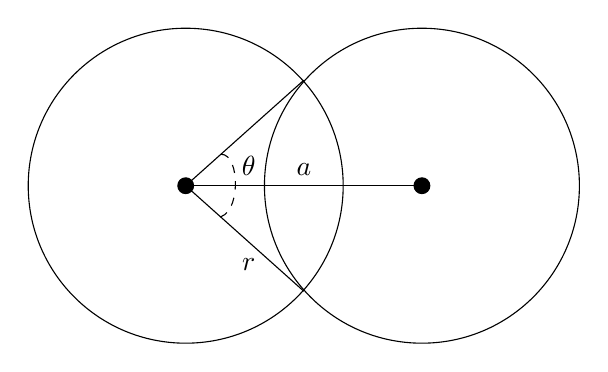
\begin{tikzpicture}
\draw (-1.5,0) circle(2);
\draw[fill=black] (-1.5,0) circle(0.1);
\draw (1.5,0) circle(2);
\draw[fill=black] (1.5,0) circle(0.1);
\draw (-1.5,0) -- (0,1.34);
\draw (-1.5,0) -- (0,-1.34);
\draw[line width=0.4,style=dashed] (-1.05,0.4) ..
controls (-0.8,0.4) and (-0.8,-0.4) .. (-1.1,-0.4);
\draw (-1.5,0) -- (1.5,0);
\coordinate [label=above:$\theta$] (A) at (-0.7,0);
\coordinate [label=above:$r$] (A) at (-0.7,-1.2);
\coordinate [label=above:$a$] (A) at (0,0);
\end{tikzpicture}
\\
Cells are composed of two overlapping circles. When the cell is in Interphase, the axis $a$ connecting the cell centers is zero, thus the cell is a single circle with a radius $r$. The cell progresses through Interphase by increasing the size of $r$ from $r_{min}$ to $r_{max} = \sqrt{2}r_{min}$, thus doubling it's area. When the cell in is Mitosis, the axis $a$ grows from 0 to $2r_{min}$, and at that point the cell divides and two daughter cells, each with the minimum radius, are created. During Mitosis the area of the cell is fixed, so as the axis expands, the radius of each cell component shrinks. $r$ and $a$ are related through $\theta$ as follows:\\
\\
Let $V$ be the volume of the dumbell:\\
\\
$a = 2r\cos(\theta /2)$\\
\\
$\frac{1}{2}V = \dfrac{2\pi - \theta}{2\pi} \pi r^2 +
\dfrac{r\cos(\theta / 2)2r\sin(\theta / 2)}{2}$\\
\\
$V = r^2(2\pi - \theta) + 2r^2\sin(\theta / 2)\cos(\theta / 2)
= r^2(2\pi - \theta + \sin(\theta))$\\
\\
$r = \sqrt{\dfrac{V}{2\pi - \theta + \sin(\theta)}}
= \dfrac{a}{2\cos(\theta / 2)}$\\
\\
\\
$a = \dfrac{2\sqrt{V}\cos(\theta / 2)}{\sqrt{2\pi - \theta
		+ \sin(\theta)}}$\\
\\
So when we stretch $a$, we can solve for $\theta$ since $V$ is fixed, and once we know $\theta$ we can solve for $r$.\\
\\
\subsection{Fixed Parameter Value Derivation}
Here we explore the possible values for each of the fixed parameters that are determined based on the input parameters given above.\\
\\
\textbf{Maximum Deformation, $\Delta a_{max}$}\\
\\
We assume mitosis takes a small fixed amount of time on average, in the model we set this time to 2 hours. The axis must deform from twice the max radius to four times the minimum radius, $4r_{min} - 2r_{max} = 4r_{min} - 2r_{min}\sqrt{2} = 2r_{min}(2 - \sqrt{2})$. It must cover this distance in two hours and only can deform once per $n_g$ steps on average. Each deformation value is sampled from $Uniform(0, \Delta a_{max})$, and so on average each deformation is $\Delta a_{max} / 2$.\\
\\
$2 = \Delta t n_g \dfrac{2r_{min}(2 - \sqrt{2})}{\Delta a_{max} / 2}$\\
\\
$\Delta a_{max} = 2\Delta t n_g r_{min}(2 - \sqrt{2})$\\
\\
\textbf{Maximum Radius Growth, $\Delta r_{max}$}\\
\\
The maximum radius growth follows the same derivation as $\Delta a_{max}$ except the distance covered is $r_{max} - r_{min} = \sqrt{2}r_{min} - r_{min} = r_{min}(\sqrt(2) - 1)$. Let the cycle length be $T$ hours, then the relation is:\\
\\
$T - 2 = \dfrac{\Delta t n_g r_{min}(\sqrt(2) - 1)}{\Delta r_{max} / 2}$\\
\\
$\Delta r_{max} = \dfrac{2\Delta t n_g r_{min}(\sqrt(2) - 1)}{T - 2}$\\
\\
\textbf{Maximum Translation, $\Delta \vec{r}_{max}$}\\
\\
This is the maximum amount the position of the cell can move in a single update. We set $\Delta \vec{r}_{max} = \delta / 2$ so that if cells are in an ideal configuration we will not propose any translations that will be automatically rejected due to overlap. The ideal configuration of cells is when all cells are $\delta / 2$ apart from each other.\\
\\
\textbf{Maximum Rotation, $\Delta \gamma_{max}$}\\
\\
Similar to the maximum translation bound, we don't want a rotation to be rejected when the cells are in an ideal configuration. To achieve this we limit the rotation angle so the center of either cell will not move more than $\delta/2$. Let $\gamma$ be the angle of rotation around the center of the dumbbell\\
\\
$\dfrac{a^2}{4}  + \dfrac{a^2}{4} - 2\dfrac{a}{2}\dfrac{a}{2}\cos(\Delta\gamma) \le \dfrac{\delta^2}{4} \implies \dfrac{a^2}{2} - \dfrac{a^2}{2}\cos(\Delta\gamma) \le \dfrac{\delta^2}{4} \implies 1 - \cos(\Delta\gamma) \le \dfrac{\delta^2}{2a^2} \implies \cos(\Delta\gamma) \ge 1 - \dfrac{\delta^2}{2a^2}$\\
\\
The axis length of a cell is bounded above by $2 r_{min}$, so\\
\\
$\cos(\Delta\gamma) \ge 1 - \dfrac{\delta^2}{8r_{min}^2}$\\
\\
Since $\delta < r_{min}$ we know the right hand side is within $[0,\pi]$ and $\cos$ is decreasing on this interval, thus\\
\\
$\Delta\gamma \le \cos^{-1}\biggr(1 - \dfrac{\delta^2}{8r^2_{min}}\biggr)$\\
\\
\textbf{Time Increment, $\Delta t$}\\
\\
The model has an internal time step that specifies how much time in model hours elapses for each update step. There are two restrictions on the time increment, the growth and deformation of cells cannot move the cell more than $\delta / 2$, otherwise cells in an ideal configuration could have a growth trial rejected - which should never happen.\\
\\
$\Delta a_{max} / 2 \le \delta / 2 \implies \Delta t n_g r_{min}(2 - \sqrt{2}) \le \delta / 2 \implies \Delta t \le \dfrac{\delta}{2 n_g r_{min}(2 - \sqrt{2})}$\\
\\
$\Delta r_{max} \le \delta / 2 \implies \dfrac{2\Delta t n_g r_{min}(\sqrt(2) - 1)}{T - 2} \le \delta / 2 \implies \Delta t \le \dfrac{\delta(T - 2)}{4 n_g r_{min}(\sqrt{2} - 1)}$\\
\\
Note that $r_{min}$ and $T$ are specific to the cell type, so when setting the time increment in the model it is neccesary to use the smallest values from among all cell types. For convenience, we set the smallest $r_{min}$ to 1 and adjust all other cell sizes accordingly.\\
\\
\end{document}
\grid
\grid
\grid
